\chapter{Image processing concepts \& techniques}
\label{sec:chap4}

\section{Texture in medical images}
The texture is a variation of data at scales smaller than the scales of interest. For example, if we take an MR image from the human brain, any variation in the gray values of the imaged brain may be thought of as texture. Sometimes variation due to noise may be considered as texture. The texture is an intrinsic property of an image, and it is a valuable cue to recognize an object in the image.

The most important characteristic of texture is that it is scale-dependent. In other words, different types of textures are visible at different scales. For example, if we look at a section of the brain through a microscope, we will see a different structure of the tissue than sulci monitored. So, to use texture for identifying different types of tissue, we should be able to measure image texture in a repeatable and reliable way. In other words, it is necessary to characterize texture in an objective way, independent of human perception and visual abilities.

Structural or statistical methods may characterize texture. A structural method identifies a texture primitive pattern, and this pattern is repeated to create the viewed appearance. This approach is also known as grammars for texture description. Usually, structure methods are less common in biomedical applications. The other types of methods are statistical approaches, and they are more attractive. Figure \ref{fig14} shows how natural the transition from deterministic methods to statistical methods is. In this figure, we may easily infer from the first case in the left that a possible texture would be one surrounded by four 0s according to the other neighboring positions. But in the second case, we can see, in 7 out of 12 points, the arrangement of four 0s indicates a 1 in the middle, while in the remaining 5 cases, it indicates a 2. So the missing value has a probability of 58\% to be one and a chance of 42\% to be 2. This method is known as Markov Random Field (MRF) modeling.

\begin{figure}[htbp]
	%\resizebox{\linewidth}{!}{
	\centering 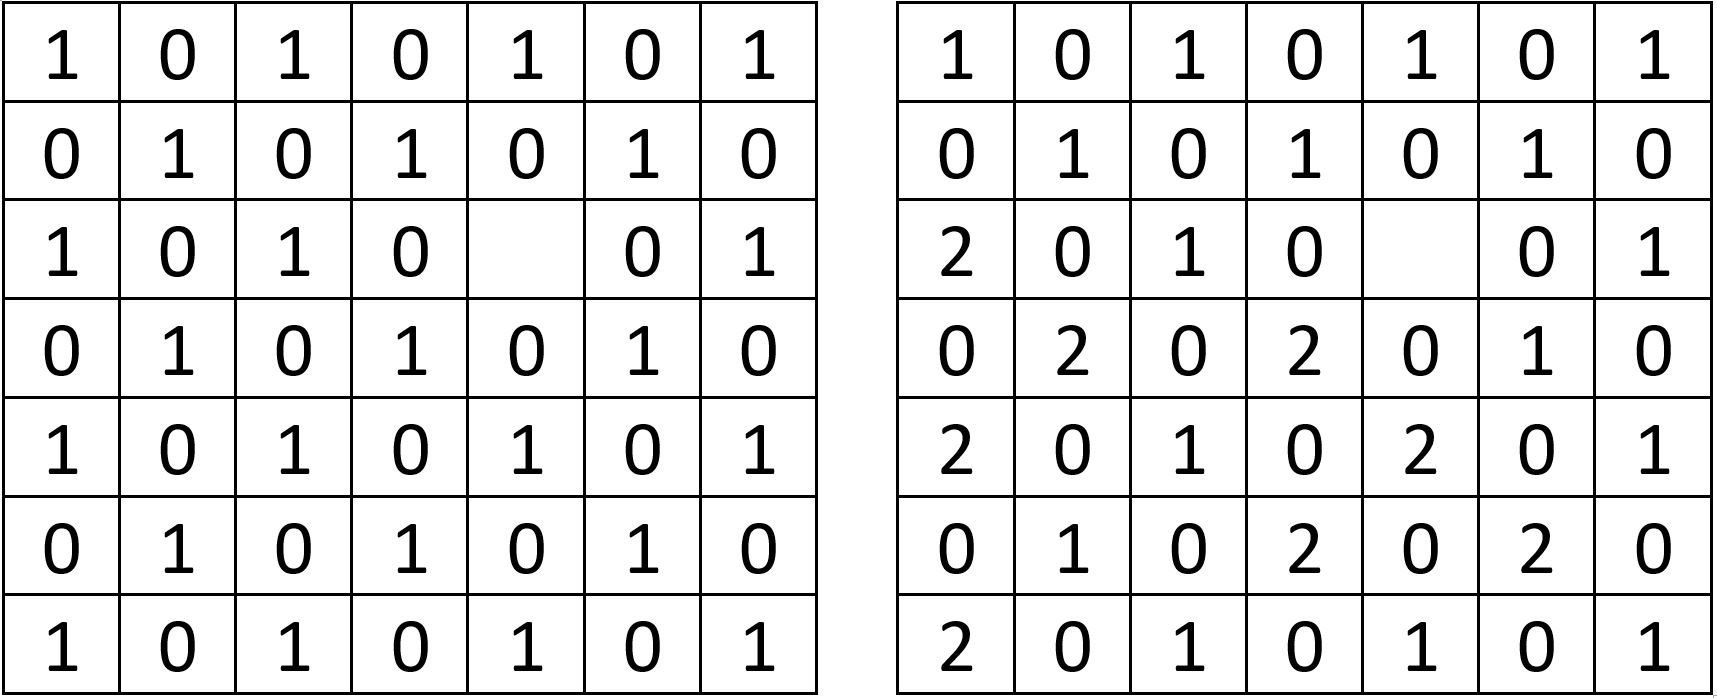
\includegraphics[width=0.6\columnwidth]{./figures/Fig14.jpg}
	\caption{Optical PET imaging instrument}
	\label{fig14}
\end{figure}

In MRF, we model the probability with which the neighbors' values are used to characterize the texture. As the statistics have to be performed on neighbor value combinations, and as pixels, particularly in medical images, take up many gray values, one needs an extensive sample of the texture to work out these parameters.

One of the issues in MRF texture approaches is the definition of the size of the neighborhood. In the previous example, we considered the smallest possible neighborhood. However, the neighborhood may be much larger to include pixels further away from the focal pixel. In the extreme case, all other pixels in the image are thought of as neighbors. In other words, the value of a pixel is directly influenced by all of the other pixels, and all scales of influence are essential.

In MRF texture descriptors, each pixel's value depends on the values of the neighbors, which have values that depend on their neighbors, and so on. The fractal models model this global dependence \textbf{explicitly}, while MRF models this global dependence \textbf{implicitly}. So, the MRF formulation leads to a formulation that models the \textbf{joint} probability density function of a particular combination of values of the whole image. Indeed, under certain conditions, an MRF modeling is equivalent to a Gibbs modeling.

Gibbs model is called clique potentials. A clique is a set of grid positions that are neighbors of each other according to the Markov model, therefore, directly influence each other’s value according to this model. In figure 10, the only cliques one can have are pairs of pixels next to each other, either vertically or horizontally. In Gibbs formalism, some parameters multiply the difference of the pairs of values of neighboring pixels to express their dependence. These parameters characterize the texture.

Gibbs distributions are not very useful in texture descriptions. However, they are beneficial in other problems of medical image processing, such as image restoration or image matching. What is important to us is how to move from local description (neighborhood-dependent modeling) to a global (joint probability).

Another noticeable transform before proceeding to quantify texture is to transform the image to the spatial frequency domain. The Discrete Fourier Transform (DFT) identifies the content of an image. DFT is complex but usually adopts its magnitude, which is known as the power spectrum. The power spectrum helps us to identify the periodicities are present in the texture.  

If we want to analyze the frequency content of the image in terms of different frequency ranges (bands), it is necessary to isolate bands in the frequency domain. Band isolation can be done with the help of some window centered at a particular frequency, and it will separate the required band. The most commonly used window is the \textbf{Gaussian} because it does not create artifacts in the image. Figure \ref{fig15} illustrates the process of band isolation.

\begin{figure}[htbp]
	%\resizebox{\linewidth}{!}{
	\centering 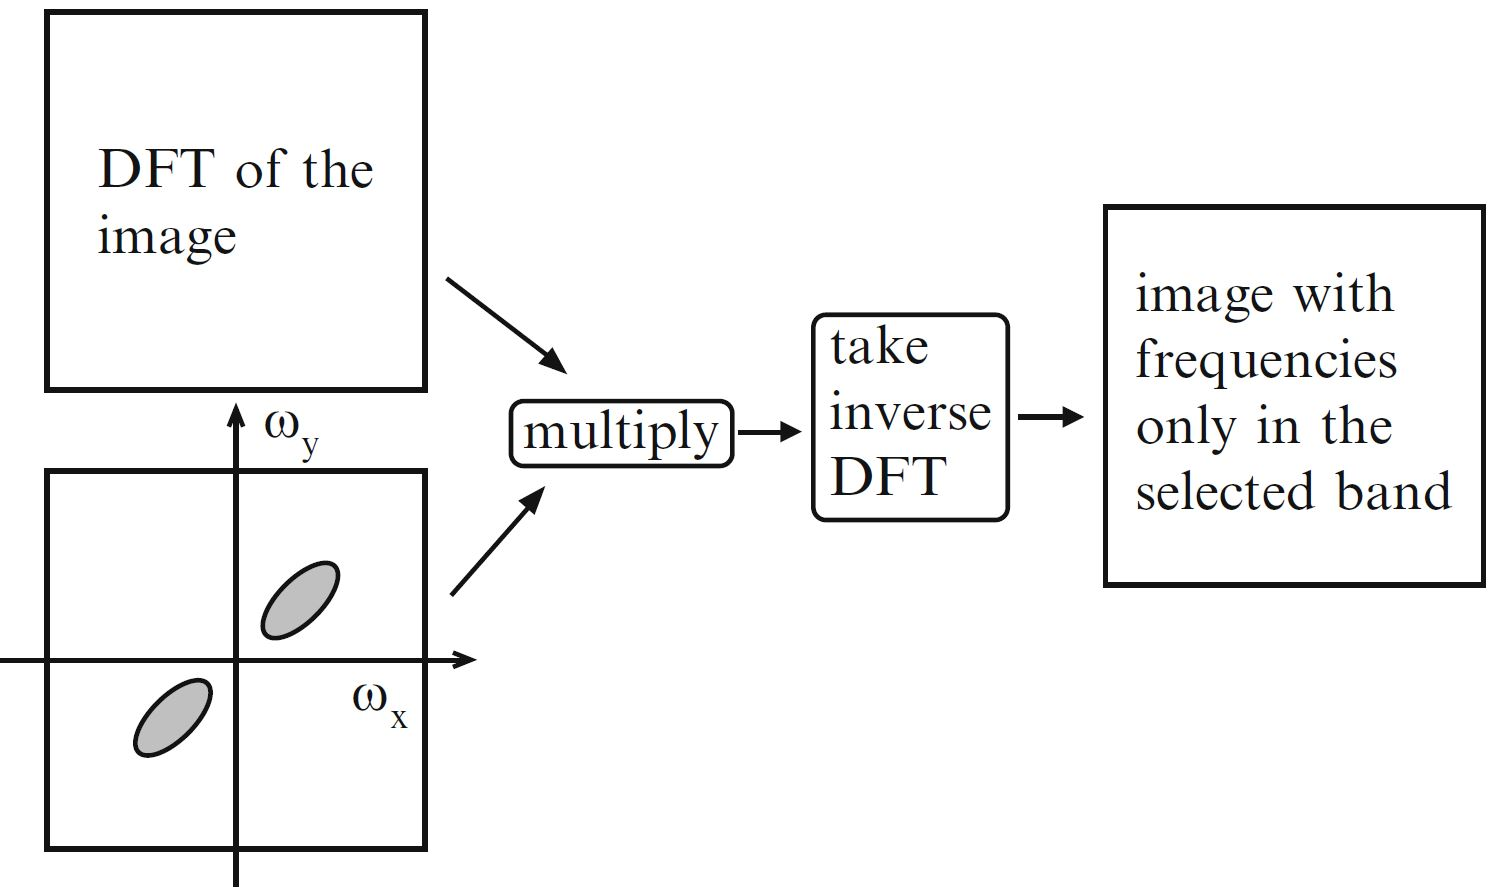
\includegraphics[width=0.6\columnwidth]{./figures/Fig15.jpg}
	\caption{Optical PET imaging instrument}
	\label{fig15}
\end{figure}

After extracting selected bands, we can compute features from them to characterize texture. The most helpful feature is the sum of the squares of the values of the output image. This feature is to find its energy in the particular frequency band.


\section{Segmentation}

The segmentation purpose is to split the image into parts, which are specific applications. The quality of the image segmentation scheme is estimated according to factors like Similarity Index, Dice Score, Sensitivity or Overlap fraction, Extra Fraction, Specificity, and Accuracy. For example, the Similarity Index (SI) tells about the mutual value among input MRI brain images and segmented output images. Accuracy is cast off to estimate the accomplishment of the tumor detection and segmentation system.

In medical imaging, segmentation often refers to the explanation of specific structures. So, it includes details of classification methods. Segmentation strategies in medical imaging combine data knowledge with domain knowledge to arrive at the result. Data knowledge refers to assumptions about continuity, homogeneity, and local smoothness of image features within segments. Domain knowledge represents information about the objects to be delineated.

Quantitative analysis of medical images requires objects or object features in the image to be identified. First, the image is segmented into regions that are the possible candidates of objects. This is followed by assigning meaning to these regions. For analyzing a digital photograph, \textbf{the segmentation} task would group pixels to areas that may belong to parts of objects based on the attributes of these regions. Hence, segmentation of images is similar to creating phonemes in speech or detecting syllables in written text. It means that the segmentation of images creates basic semantic entities from images.

However, it isn't easy to apply domain knowledge about objects in an image to segmentation. The purpose of segmentation is to create semantic entities in the first place. After segmentation, every pixel is assigned to exactly one segment since every location in an image carries just one meeting. The problem is appearances of objects in some images may be very different within and between objects classes. For example, Figure \ref{fig16} is a set of pictures contain a landscape with a house in the foreground, some trees and mountains in the background.

\begin{figure}[htbp]
	%\resizebox{\linewidth}{!}{
	\centering 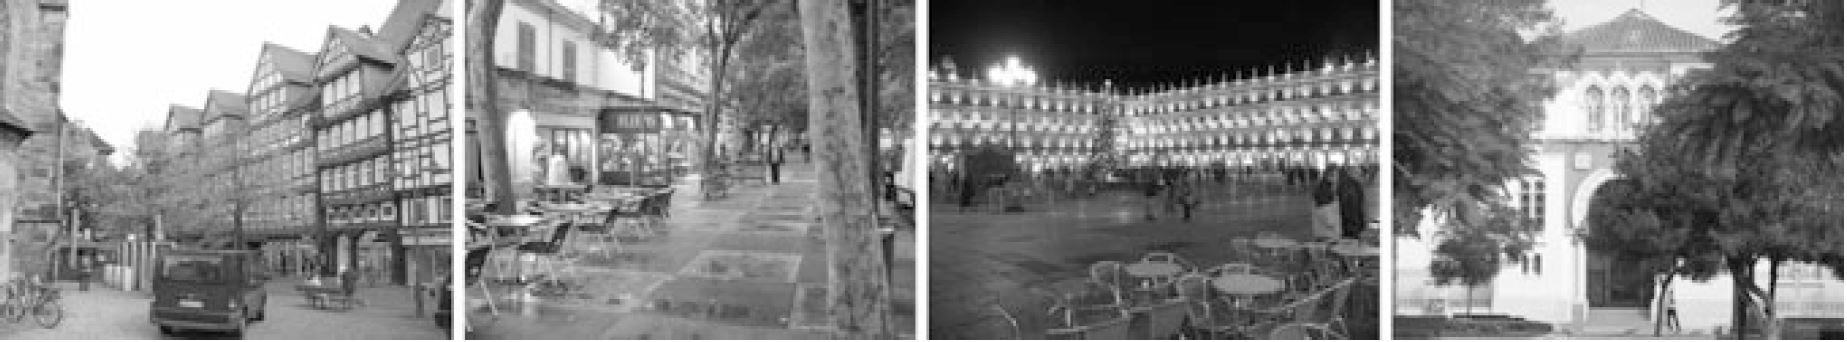
\includegraphics[width=0.7\columnwidth]{./figures/Fig16.jpg}
	\caption{Finding a general solution (find  houses) for a segmentation task}
	\label{fig16}
\end{figure}

For the segmentation of medical images, the situation is even worse, as a medical image represents the measurement of a diagnostically relevant entity measured in the same way everywhere in the body. For instance, consider a CT where X-ray attention is calculated on the normalized Hounsfield scale. Attention should not vary with location but only with density and atomic number.


There are several ways to deal with missing information without missing the assumption that a low-level segmentation criterion is valid everywhere in the image.

\textbf{Foreground segmentation} focuses on a single object in the image. Segmentation criteria create an excellent partitioning of foreground objects, whereas the quality of partitioning the background is irrelevant. The strategy requires some model knowledge to be applied after segmentation for separating foreground segments from the background. A simple way to introduce the model would be let the user point out foreground segments. Figure \ref{fig17} is an example of segmenting liver in a CT image.

\begin{figure}[htbp]
	%\resizebox{\linewidth}{!}{
	\centering 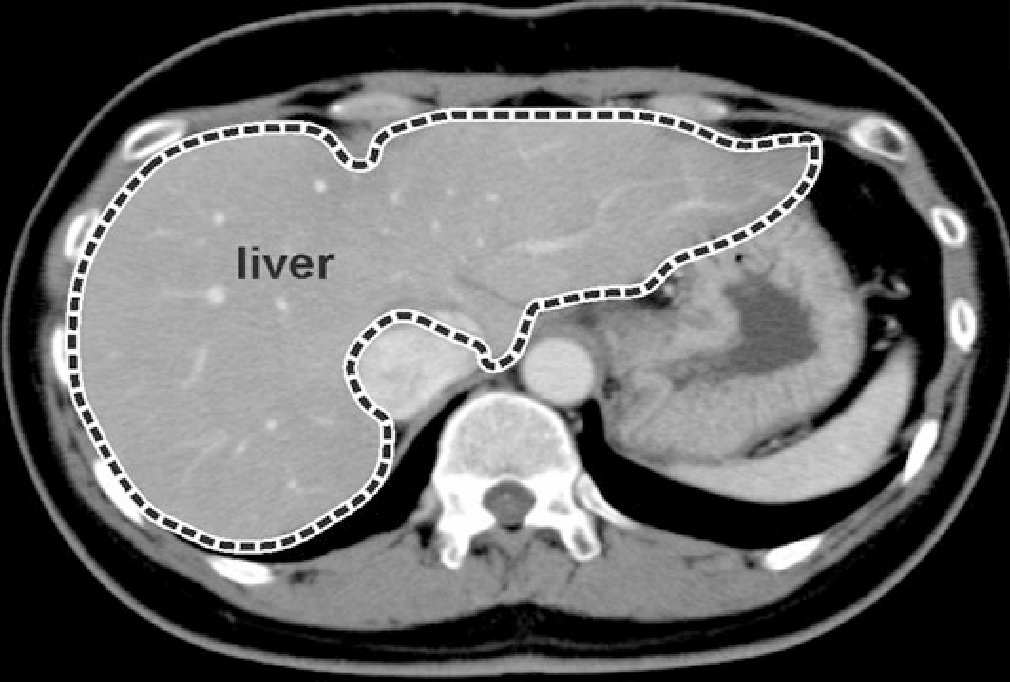
\includegraphics[width=0.6\columnwidth]{./figures/Fig17.jpg}
	\caption{Segmentation of liver from all other tissues}
	\label{fig17}
\end{figure}

\textbf{Hierarchical segmentation} (Figure \ref{fig18}) applies a multi-resolution concept for gradual refinement. A first segmentation creates segments that are smaller than the smallest object. It is assumed that a common criterion can be found at this scale. The result is sometimes called over-segment. Some of these segments are merged into larger segments at the next level according to domain knowledge about object appearance. Successful application of this strategy requires that common criteria define meaningful segments at a single but unknown scale. This scale is found by analyzing the levels of the segmentation hierarchy.


\begin{figure}[htbp]
	%\resizebox{\linewidth}{!}{
	\centering 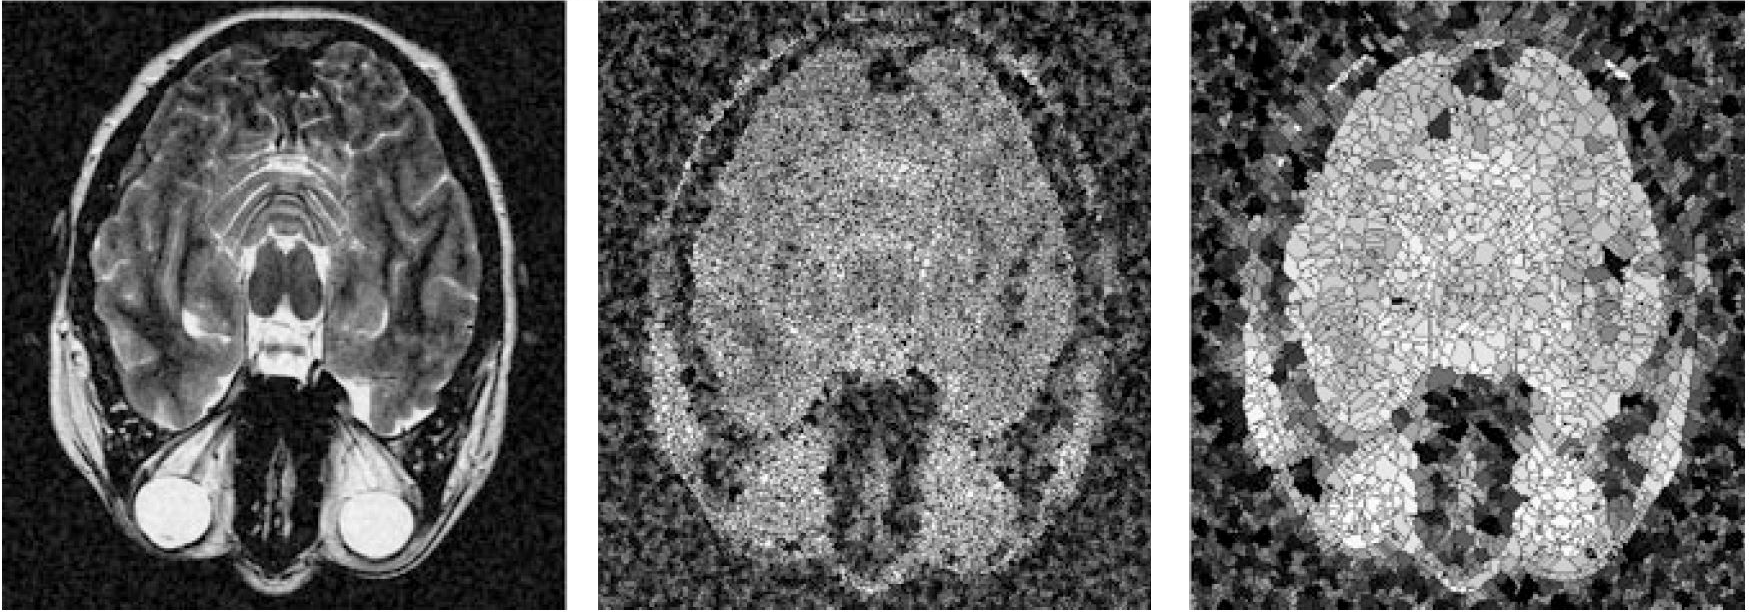
\includegraphics[width=0.55\columnwidth]{./figures/Fig18.png}
	\caption{hierarchical segmentation different stages}
	\label{fig18}
\end{figure}

\textbf{Multilayer segmentation} is another multi-resolution technique. It is assumed that a common segmentation criterion exists but that its scale may vary throughout the image (like the structured texture of an object in which the scale varies with the distance of the object to the camera). Segmentation is carried out at different scales producing layers of segments. Multilayer segmentation is more general than the previous strategy. The criterion scale often varies because an appropriate scale for every segment has to be established independently from other segments. Figure \ref{fig19} illustrates steps of multilayer segmentation. 

\begin{figure}[htbp]
	%\resizebox{\linewidth}{!}{
	\centering 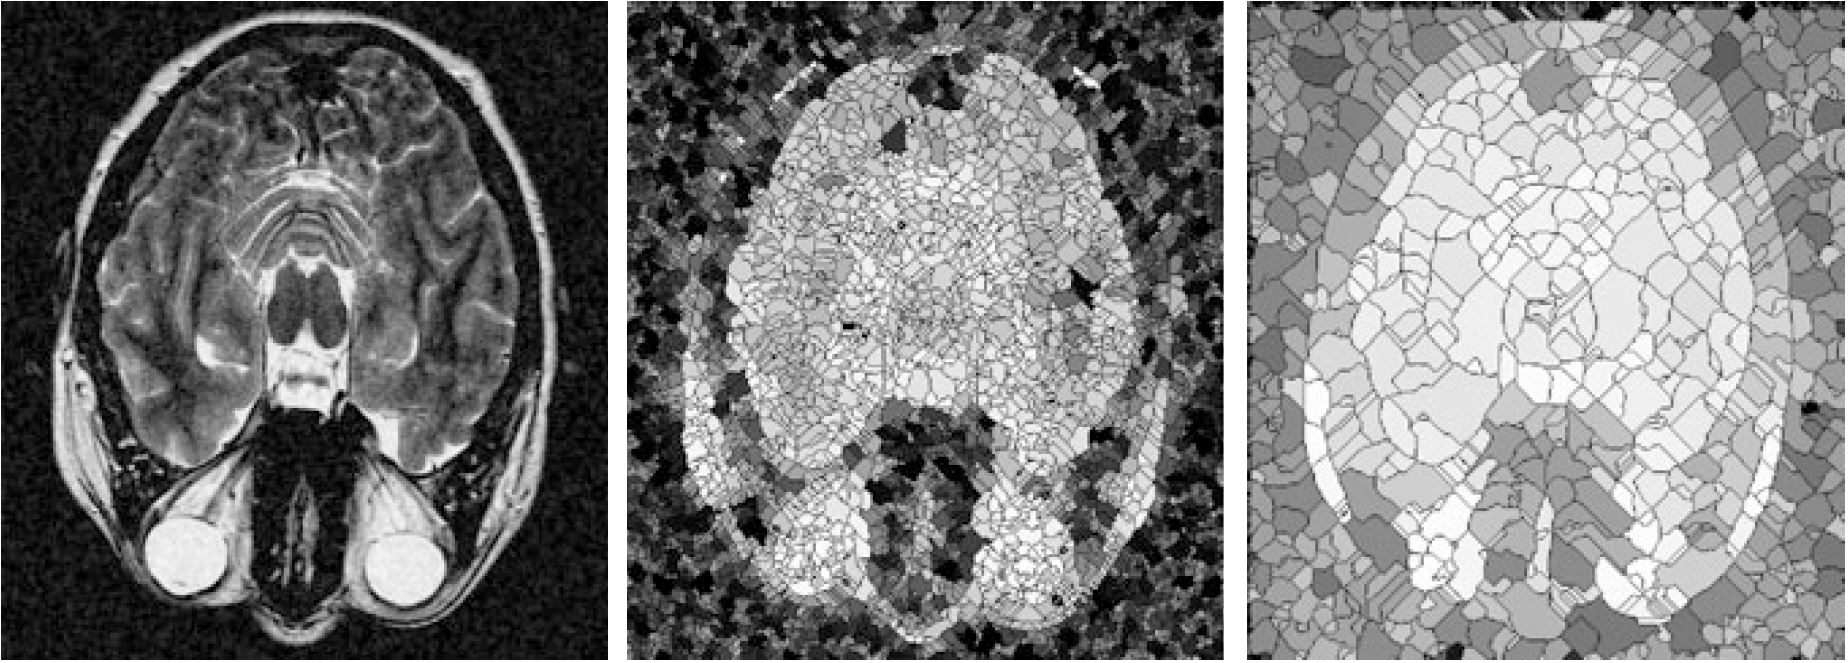
\includegraphics[width=0.55\columnwidth]{./figures/Fig19.png}
	\caption{segmentation at different levels of resolution are evaluated in parallel}
	\label{fig19}
\end{figure}

The search for a specific structure by segmentation causes foreground segmentation to be more frequent in medical image analysis than in other image analysis tasks. Since it may involve a detection task, a model-driven approach then discriminates the structure from the background. Model knowledge may be integrated into the algorithm or supplemented interactively. Popular segmentation techniques, such as the various region growing, active contours and surfaces, and active shape models, use a model-driven approach.

\section{Thresholding}

Thresholding is the simplest method of image segmentation. Various thresholding techniques are:
\begin{enumerate}
	\item \textbf{Global Thresholding}: In this method, we use a bimodal image. A bimodal image is an image with 2 peaks of intensities in the intensity distribution plot. One for the object and one for the background. Then we deduce the threshold value for the entire image and use that global threshold for the whole image. A disadvantage of this type of threshold is that it performs really poorly during poor illumination in the image(Figure \ref{fig21}).
	
	\begin{figure}[htbp]
		%\resizebox{\linewidth}{!}{
		\centering 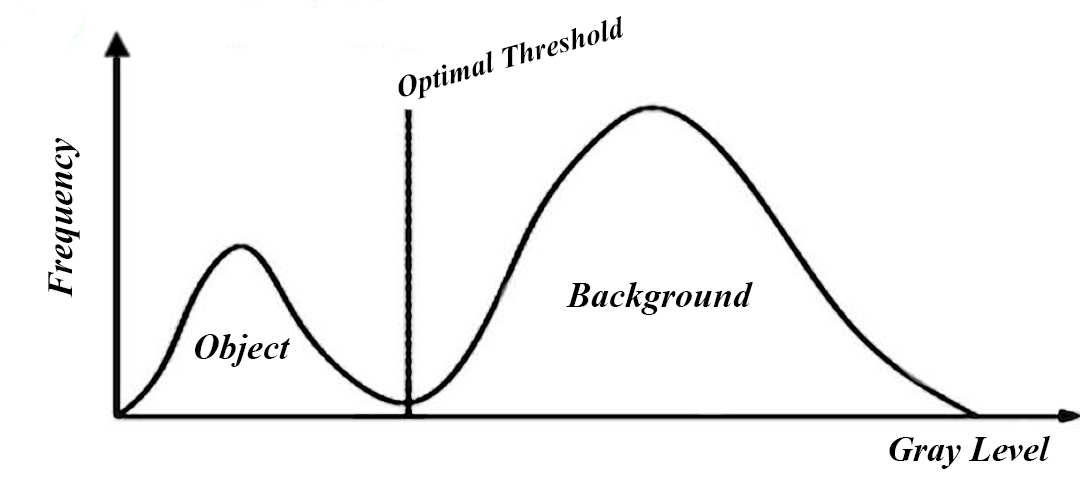
\includegraphics[width=0.55\columnwidth]{./figures/Fig21.jpg}
		\caption{Global Thresholding}
		\label{fig21}
	\end{figure}
	
	\item \textbf{Multimodal Thresholding}: A general approach to thresholding is based on assumption that images are multimodal, that is, different objects of interest relate to distinct peaks (or modes) of the 1D signal histogram. The thresholds have to optimally separate these peaks in spite of typical overlaps between the signal ranges corresponding to individual peaks(Figure \ref{fig22}).
	
	\begin{figure}[htbp]
		%\resizebox{\linewidth}{!}{
		\centering 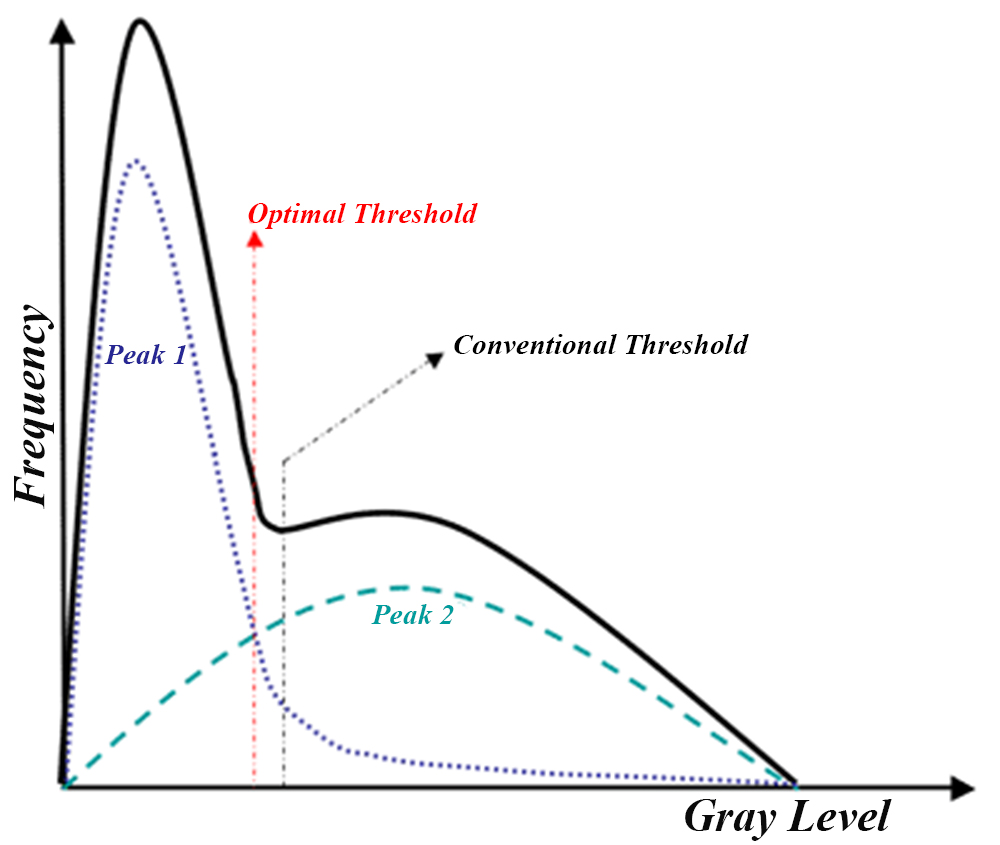
\includegraphics[width=0.55\columnwidth]{./figures/Fig22.jpg}
		\caption{Multimodal Thresholding}
		\label{fig22}
	\end{figure}
	
	\item \textbf{Adaptive Thresholding}: The image is divided into various subregions, and all these regions are segmented using the threshold value calculated for all these regions. Then these subregions are combined to image the complete segmented image. This helps in reducing the effect of illumination to a certain extent.
	
\end{enumerate}



\section{Artificial Neural Network}

ANN stands for Artificial Neural Network. Just like humans have BNN i.e. the Biological Neural Network, the researchers tried to replicate the working of the human brain and came up with the great invention of an Artificial Neural Network. ANNs have been developed for a wide range of applications such as function approximation, feature extraction, optimization, and classification. In particular, they have been developed for image enhancement, segmentation, registration, feature extraction, and object recognition.

There are three types of learning in ANN. They are supervised learning, unsupervised learning and reinforced learning. \textbf{Supervised learning} is based on error between output and input data. A teacher or supervisor is offered during learning process and offered projected output. In \textbf{Unsupervised learning} no teacher is presented to teach to the network. Unsupervised learning is very complex and difficult to implement. The system learns of its own by discovering and adapting to the structural features in the input sample of data. \textbf{Reinforced learning} is output based learning. Although a teacher existed during the procedure but, the teacher is not going to present the actual output. The teacher only indicated whether the output is correct or incorrect.

\section{Clustering}
Clustering is a type of unsupervised machine learning algorithm. It is highly used for the segmentation of images. One of the most dominant clustering-based algorithms used for segmentation is KMeans Clustering. This type of clustering can be used to make segments in a colored image. Three main clustering methods are as follows:

\begin{enumerate}
	\item \textbf{Traditional Clustering}
	\item \textbf{Hierarchical Clustering}: Also called Hierarchical cluster analysis or \textbf{HCA} is an unsupervised clustering algorithm. The algorithm groups similar objects into groups called clusters. The endpoint is a set of clusters that have ordering from top to bottom.
	\item \textbf{Partitional Clustering}: These algorithms minimize a given clustering criterion by iteratively relocating data points between clusters until a (locally) optimal partition is attained. Famous \textbf{K-means clustering} comes under partitioning method.
\end{enumerate} 


\section{Edge Detection}

Edge-based segmentation relies on edges found in an image using various edge detection operators. These edges mark image locations of discontinuity in gray levels, color, texture, etc. When we move from one region to another, the gray level may change. So if we can find that discontinuity, we can find that edge. This process detects outlines of an object and boundaries between objects and the background in the
image. An edge-detection filter can also be used to improve the appearance of blurred image. A variety of edge detection operators are available but the resulting image is an intermediate segmentation result and should not be confused with the final segmented image. We have to perform further processing on the image to the segment it. Additional steps include combining edges segments obtained into one segment in order to reduce the number of segments.

Edges are usually associated with “Magnitude” and “Direction”. Some edge detectors give both directions and magnitude. We can use various edge detectors like Sobel edge operator, canny edge detector, Kirsch edge operator, Prewitt edge operator, Robert’s edge operator, etc.

\section{Region-Based}
A region can be classified as a group of connected pixels exhibiting similar properties. The similarity between pixels can be in terms of intensity, color, etc. In this type of segmentation, some predefined rules are present which have to be obeyed by a pixel in order to be classified into similar pixel regions. Region-based segmentation methods are preferred over edge-based segmentation methods in case of a noisy image. Region-Based techniques are further classified into 3 types based on the approaches they follow.

\begin{enumerate}
	\item \textbf{Region Growing}: We start with some pixel as the seed pixel and then check the adjacent pixels. If the adjacent pixels abide by the predefined rules, then that pixel is added to the region of the seed pixel and the following process continues till there is no similarity left.
	\item \textbf{Region Splitting}: The whole image is first taken as a single region. If the region does not follow the predefined rules, then it is further divided into multiple regions (usually 4 quadrants) and then the predefined rules are carried out on those regions in order to decide whether to further subdivide or to classify that as a region. This process continues till there is no further division of regions required
	\item \textbf{Splitting \& Merging}: In these methods, after splitting regions we consider every pixel as an individual region. We select a region as the seed region to check if adjacent regions are similar based on predefined rules. If they are similar, we merge them into a single region and move ahead in order to build the segmented regions of the whole image.
\end{enumerate}


\section{Graph-Based}

graph-based methods present different graph representations, where the nodes may be pixels, pixel vertices, regions, or user-drawn markers. They also differ in the graph algorithm used to solve the problem: graph matching, random walker, the min-cut/max-flow algorithm, Dijkstra's algorithm, Kruskal's or Prim's algorithm, etc. Figure \ref{fig23} illustrates how graph-based segmentation algorithms work.

\begin{figure}[htbp]
	%\resizebox{\linewidth}{!}{
	\centering 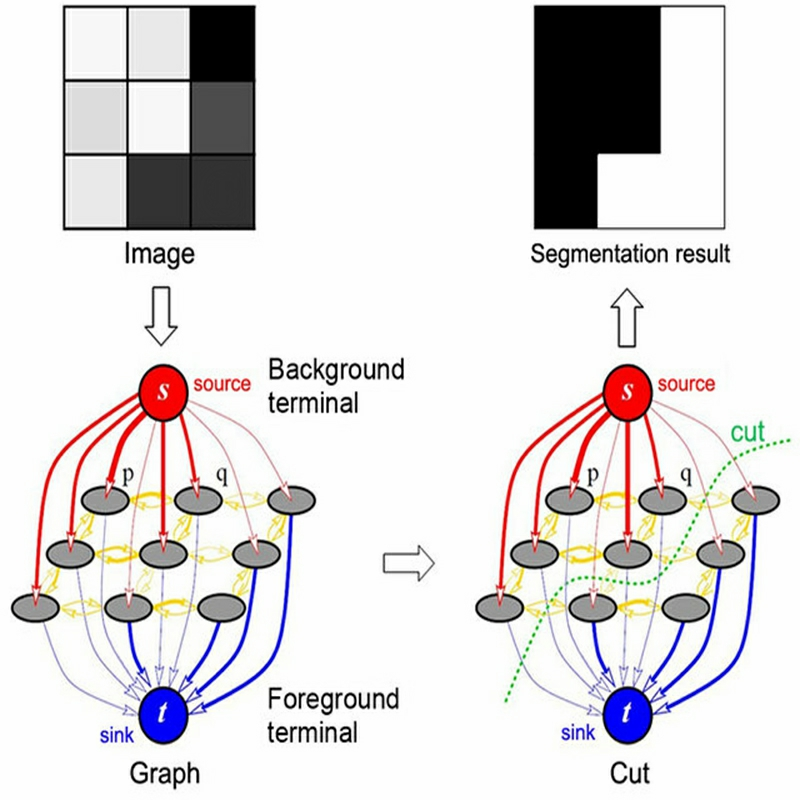
\includegraphics[width=0.65\columnwidth]{./figures/Fig23.jpg}
	\caption{Graph-based segmentation}
	\label{fig23}
\end{figure}


\section{Derformable Models}

Deformable models have been extensively studied and widely used in medical image segmentation, with promising results. Deformable
models are curves or surfaces defined within an image domain that can
move under the influence of internal forces, which are defined within the curve or surface itself, and external forces, which are computed from the image data. The internal forces are designed to keep the model smooth during deformation. The external forces are defined to move the model toward an object boundary or other desired features within an image.

\section{Watershed}
It is often used when we are dealing with one of the most difficult operations in image processing – separating similar objects in the image that are touching each other. To understand the “philosophy” behind the watershed algorithm we need to think of a grayscale image as a topographic surface. In such an image high-intensity pixel values represent peaks (white areas), whereas low-intensity values represent valleys – local minima (black areas). we start filling every isolated valley with water. the rising water from different valleys will start to merge. To avoid that, we need to build barriers in the locations where the water would merge. These barriers we call watershed lines and they are used to determine segment boundaries.


We described some of the most common strategies for segmenting medical images. Figure \ref{fig20} shows various approaches for segmentation.

\begin{figure}[htbp]
	%\resizebox{\linewidth}{!}{
	\centering 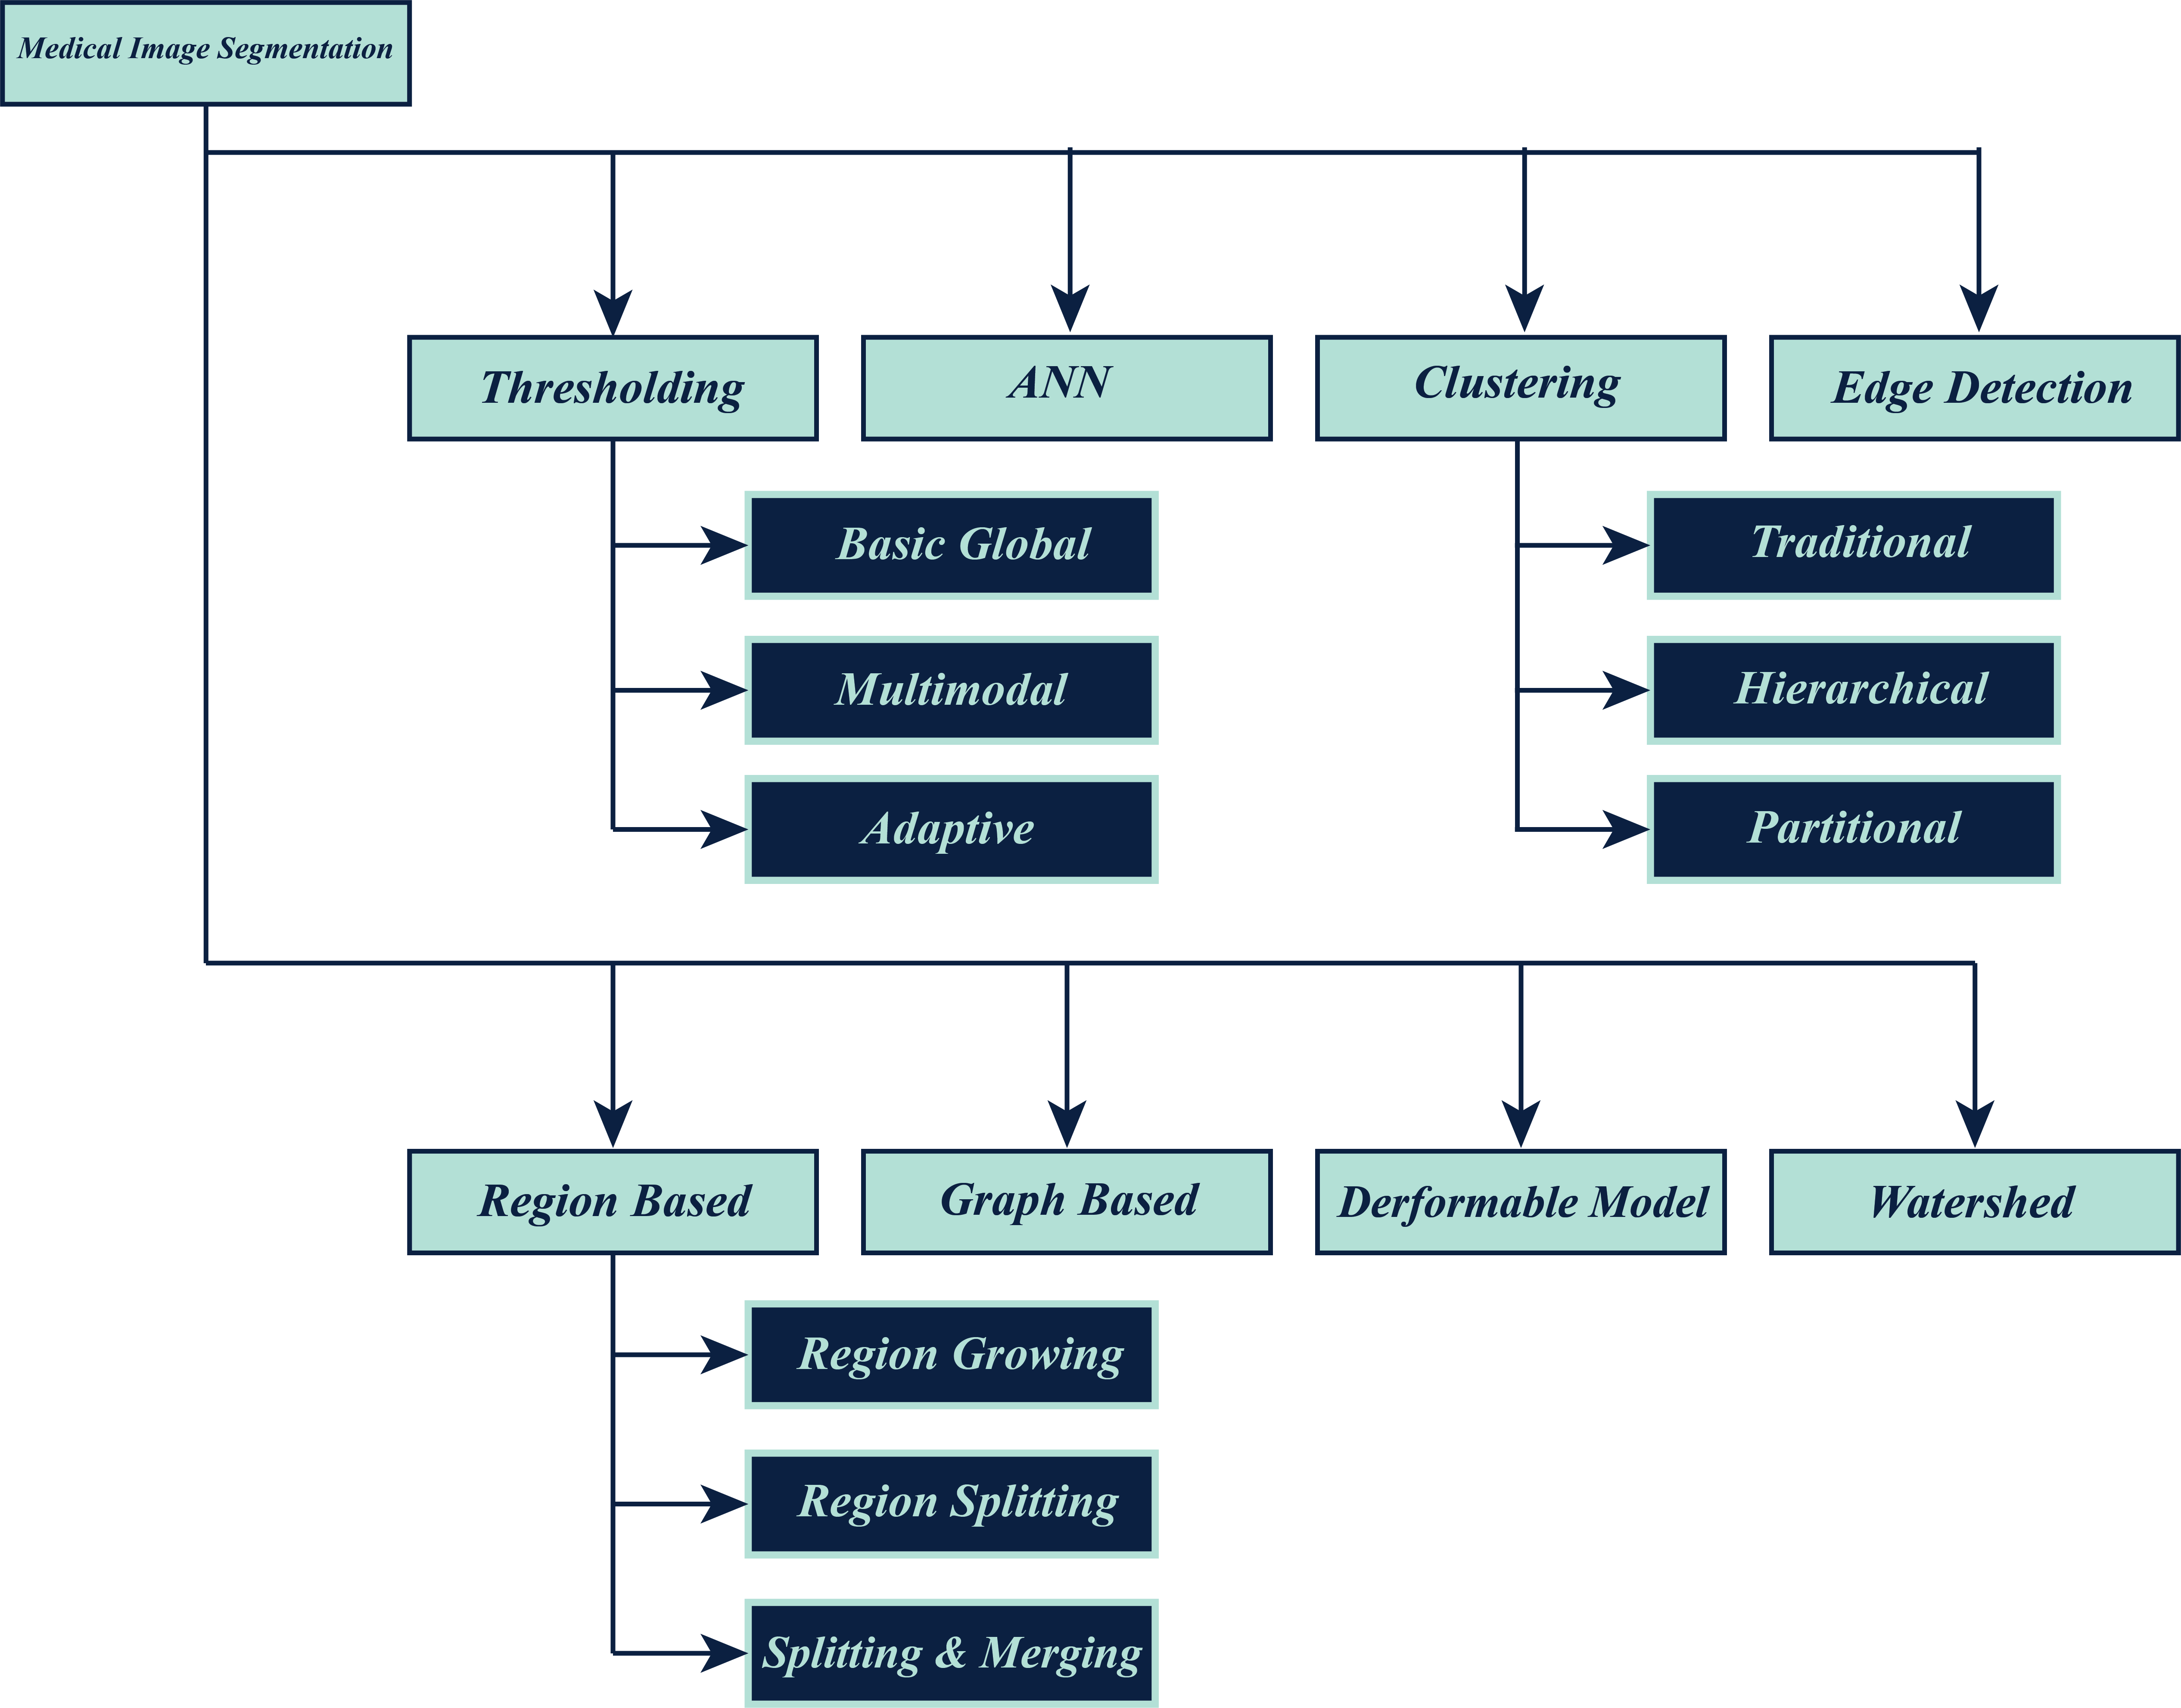
\includegraphics[width=0.75\columnwidth]{./figures/Fig20.png}
	\caption{segmentation techniques}
	\label{fig20}
\end{figure}

\section{Denoising}
Image denoising is required to use in digital image processing. From the researchers’ point of view, image denoising is still challenging task in medical images. Image denoising stays a normal process in digital image processing. It remains a pre-processing period to eradicate specific unidentified such as Additive White Gaussian Noise (AWGN) from an image to get a clean image used in favor of image processing, such as image segmentation. A representative instance of the image processor is image denoising prototypical. This method incorporates a disintegrated prototypical giving to some prior information of a corrupted image. To reestablish the distorted image in favor of obtaining a promising result. 

In this instance, \textit{$n_0$} tells about noisy medical image and $\textit{w}$ is an original, nevertheless usually known or unknown image i.e.,

\begin{equation}
	\centering
	n_0 = Dw + n_1
\end{equation}.

In which \textit{D} is a linear or non-linear operator representing the distortion and \textit{$n_1$} is additive noise.

The performance of the image denoising method is measured by using the essential factors such as Mean or Average pixel intensity, Standard Deviation, Mean Square Error, Root Mean Square Error, Mean Absolute Error, Peak Signal to Noise Ratio, Structural Similarity, Universal Image Quality Index, and Entropy. For example, the mean parameter determines the dissimilarity of the image by adding all the pixels and dividing the total pixels of the image. The average gradient gives the sharpness and clarity of the image.

There are other algorithms and general technologies designed intended for image denoising. These are listed below:

\section{Statistical modeling-based image denoising}

In 2018, Wang presented the minimax-concave TV (MCTV) to reconstruct the MR brain image. MCTV is non-convex, mainly to represent the nonconvexity parameter correctly and at the same time maintain a convexity for every iteration step.

In 2016, Park suggested a method of learning-based denoising. This method significantly reduces PI noise, and the start-up time is much faster. It creates high-quality images that do not have degrading information to increase speed. In the same year, Zhang demonstrated an MRI denoising framework that structurally correlates between users to evaluate the models efficiently to reduce noise in the signal.

\section{Derivative-based image denoising}
In 2017, Magudeeswaran developed a novel level-set technique originates from the active contour prototypical. This technique diminishes the costly initialization of a level set approach further efficiently. Primarily, images are pre-processed with the Contrast Limited Fuzzy Adaptive Histogram Equalization (CLFAHE) improvement technique to enhance the dissimilarity of the image.

In 2016, Sedaaghi solved PM flux analysis problems. In this method, the image remains bisected into three slices, depending on gradient level: the area where the slope is inferior to the smoothness of the area, where the slope is between the smoothness and the flux point, and the slope area is higher than the flux point. Also, in this year, Yang proposed an image denoising algorithm using PDE and GCV. In this method, the blocking effect is reduced by tetrolet transformation and is considered to be good.

To eradicate the staircase consequence aimed at TV filter and evading boundaries distorting in support of fourth-order PDE filter, Tan suggested the anisotropic diffusion in favor of image denoising. In this method, if the pixels are part of the flat area, a fourth-order filter is accepted that can remove the staircase artifacts. Figure \ref{fig24} illustrates these denoising methods in an abstract view.

\begin{figure}[htbp]
	%\resizebox{\linewidth}{!}{
	\centering \includegraphics[width=1\columnwidth,height=12cm]{./figures/Fig24.png}
	\caption{Image Denoising Methods}
	\label{fig24}
\end{figure}
